\section{Cascade}\label{sec:cascade}

A última etapa consiste em combinar classificadores fortes em cascata de modo a
processar eficientemente regiões da imagem em busca de um padrão. Cada estágio na cascata aplica um classificador mais específico e complexo do que o anterior, de modo que o algoritmo rejeite rapidamente regiões que sejam muito distintas da característica procurada e termine o processo de procura neste caso, evitando que os estágios posteriores sejam executados desnecessariamente. Isso faz com que muitos dos cenários e panos de fundo sejam descartados nos primeiros estágios e apenas faces e outros objetos semelhantes a faces sejam analisados mais exaustivamente \cite{refer4}. 

%\begin{comment}
\begin{figure}[ht]
\centering
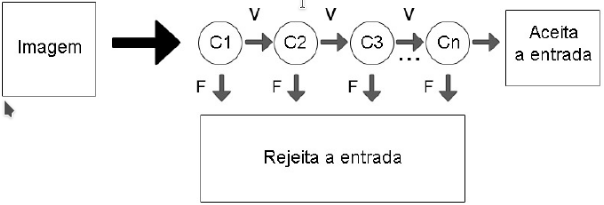
\includegraphics[width=8cm]{images/haar-cascade.png}
\caption{Seleção das imagens}
\label{fig:haar cascade}
\end{figure}

%\end{comment}
